
\part*{Kosten- und Leistungsrechnung}

Unternehmen erbringen Leistungen, diese stiften einen Nutzen, der
sich auf dem Makr verkaufen lässt (oder intern gebraucht wird).

Zielsetzung:
\begin{itemize}
\item Ermittlung der Kosten des Leistungserstellungsprozesses
\item Zurechnung der Kosten auf Leistungsträger
\item Gegenüberstellung von Nutzen und Kosten einzelner Leistungsträger
\item Bereitstellung von Kalkulationsgrundlagen für Leistungsträger
\end{itemize}

\paragraph*{Kosten}

Geld- Sachgüter- oder Dienstleistungsverbrauch für die betriebliche
Leistungserstellung.


\paragraph*{Aufwand}

Vermögensminderung oder Entstehung von Fremdkapital, die ihren Grund
im Absatz oder Herstellung von Gütern oder in der Erstellung von Dienstleistungen
haben.


\section*{Kosten - Aufwand: Abgrenzung}

Die Kosten können von den Aufwänden der Finanzbuchhaltung abgeleitet
werden.

Jedoch: 
\begin{itemize}
\item nichtbetriebliche und ausserordentliche Aufwände sind nicht als Kosten
zu betrachten
\item (Bildung und Auflösing stiller Reserven) Der tatsächliche Werteverzehr
muss ermittelt werden.
\item Verzinsungsverbot für Eigenkapital, gelegentliche Mitarbeit: mit Zusatzkosten
umschrieben
\end{itemize}

\section*{Kostenermittlung}


\paragraph*{Grundsatz}

Mit Jedem Beleg, der in der FInanzbuchhaltung einem Aufwandkonto belastet
wird, erfolgt gleichzeitig auch die Belastung des Objektes, das die
Kosten verursacht (Kostenstelle oder Kostenträger).


\paragraph*{Kostenabgrenzung}

Es können Abgrenzungsprobleme insbesondere bei den Zusatzkosten entstehen,
da diese dort ja nicht in der Finanzbuchhaltung als Aufwand verbucht
worden waren. Oder auch dann, wenn man für die Bewertung des Verbrauchs
von Sachgütern unterschiedliche Bewertungsverfahren verwendet.


\paragraph*{Ermittlung des kalkulatorischen Zinses}
\begin{quote}
\begin{tabular}{|l|>{\centering}p{7cm}|}
\hline 
\noun{Kategorie} & \noun{Beispiele}\tabularnewline
\hline 
\hline 
Summe der Aktiven (interne Werte) & \tabularnewline
\hline 
- nichtbetriebsnotwendige Aktive & \tabularnewline
\hline 
= betriebsnotwendige Aktive, Kapital & \tabularnewline
\hline 
- Abzugskapital & Fremdkapital ohne Zinskosten oder Zinskosten über anderes Konto abgerechnet\tabularnewline
\hline 
= kalkulatorisch zu verzinsendes Kapital & \tabularnewline
\hline 
\end{tabular}
\end{quote}

\paragraph*{Kalkulatorische Zinskosten}

= $\emptyset$ kalk. zu verzinsendek Kapital {*} kalk. Zinssatz


\paragraph*{Methoden zur Bewertung}
\begin{itemize}
\item First-In-First-Out (FiFo)
\item Last-In-First-Out (LiFo)
\item Highest-In-First-Out (HiFo)
\item Gleitender Durchschnitt (GLEP)
\end{itemize}

\section*{Zurechnung der Kosten}

Es kann lediglich ein Teil der Kosten \textbf{direkt} einem Leistungsträger
zugerechnet werden. Diese Kosten nennt man ``direkte Kosten'' oder
``Einzelkosten''. Dazu gehören:
\begin{itemize}
\item Material für die Herstellung (es steht fest wie viel Geldeinheiten
Material in einem Leistungsträger steckt)
\item Kosten für verbrauchte Handelswaren
\item ein Teil der Personalkosten (Lohnansatz und Zeitaufwand für die Leistung
ist ja bekannt)
\end{itemize}
Kosten, die sich nicht direkt zurechnen lassen, werden ``\textbf{indirekte}
Kosten'' oder ``Gemeinkosten'' genannt. Dazu gehören:
\begin{itemize}
\item Kosten, die durch den Einkaufsvorgang ausgelöst werden (Marktforschung,
Aufgabe der Bestellung)
\item Kosten der Lagerung (Raumkosten, Kühlgeräte)
\item Abschreibungen, Reparatur \& Unterhalt, Energieverbrauch, Kapitalkosten
\item Verpacken, Kassieren etc (kann nicht auf einzelne Leistungsträger
umgeweltzt werden)
\item Buchhaltung, Administration, Lohnabrechnung
\end{itemize}
Zurechnung der Kosten auf die Kostenstellen
\begin{itemize}
\item Personalkosten auf Kostenstelle gemäss Stundenrapport
\item Abschreibungskosten auf Kostenstelle aufgrund von Anlagekartei mit
Anschaffungswert, Alter, Abschreibungsmethode, Nutzungsdauer
\item Zinskosten auf Kostenstelle aufgrund Anlagekartei mit Kapitalbetrag
\end{itemize}
Zurechnnung der Kostenstellenkosten auf die Leistungsträger
\begin{itemize}
\item Kostenstelle ``Einkauf und Lager'': im Verhältnis zu den Einzelmaterialkosten
den Leistungsträgern zuordnen
\item Kostenstelle ``Fertigung'': durch Leistungsträger verursachte Beanspruchung
zurechnen (Maschinenstunden)
\item Kostenstelle ``Verkauf'' und ``Verwaltung'': den Leistungsträgern
im Verhältnis ihrer Herstellkosten oder Erlöse zurechnen
\end{itemize}

\paragraph*{Leistungsträgerrechnung}

Sie erlaubt uns rückblickend festzustellen, mit welchen Zuschlagssätzen
die Gemeinkosten den Leistungsträgern zugerechnet wurden. Eine solche
Kalkulation heisst ``Nachkalkulation''. Verwenden man diese rückblickend
ermittelten Kalkulationssätze um einen neuen Auftrag zu kalkulieren,
spricht man von ``Vorkalkulation''.


\section*{Beispiel}

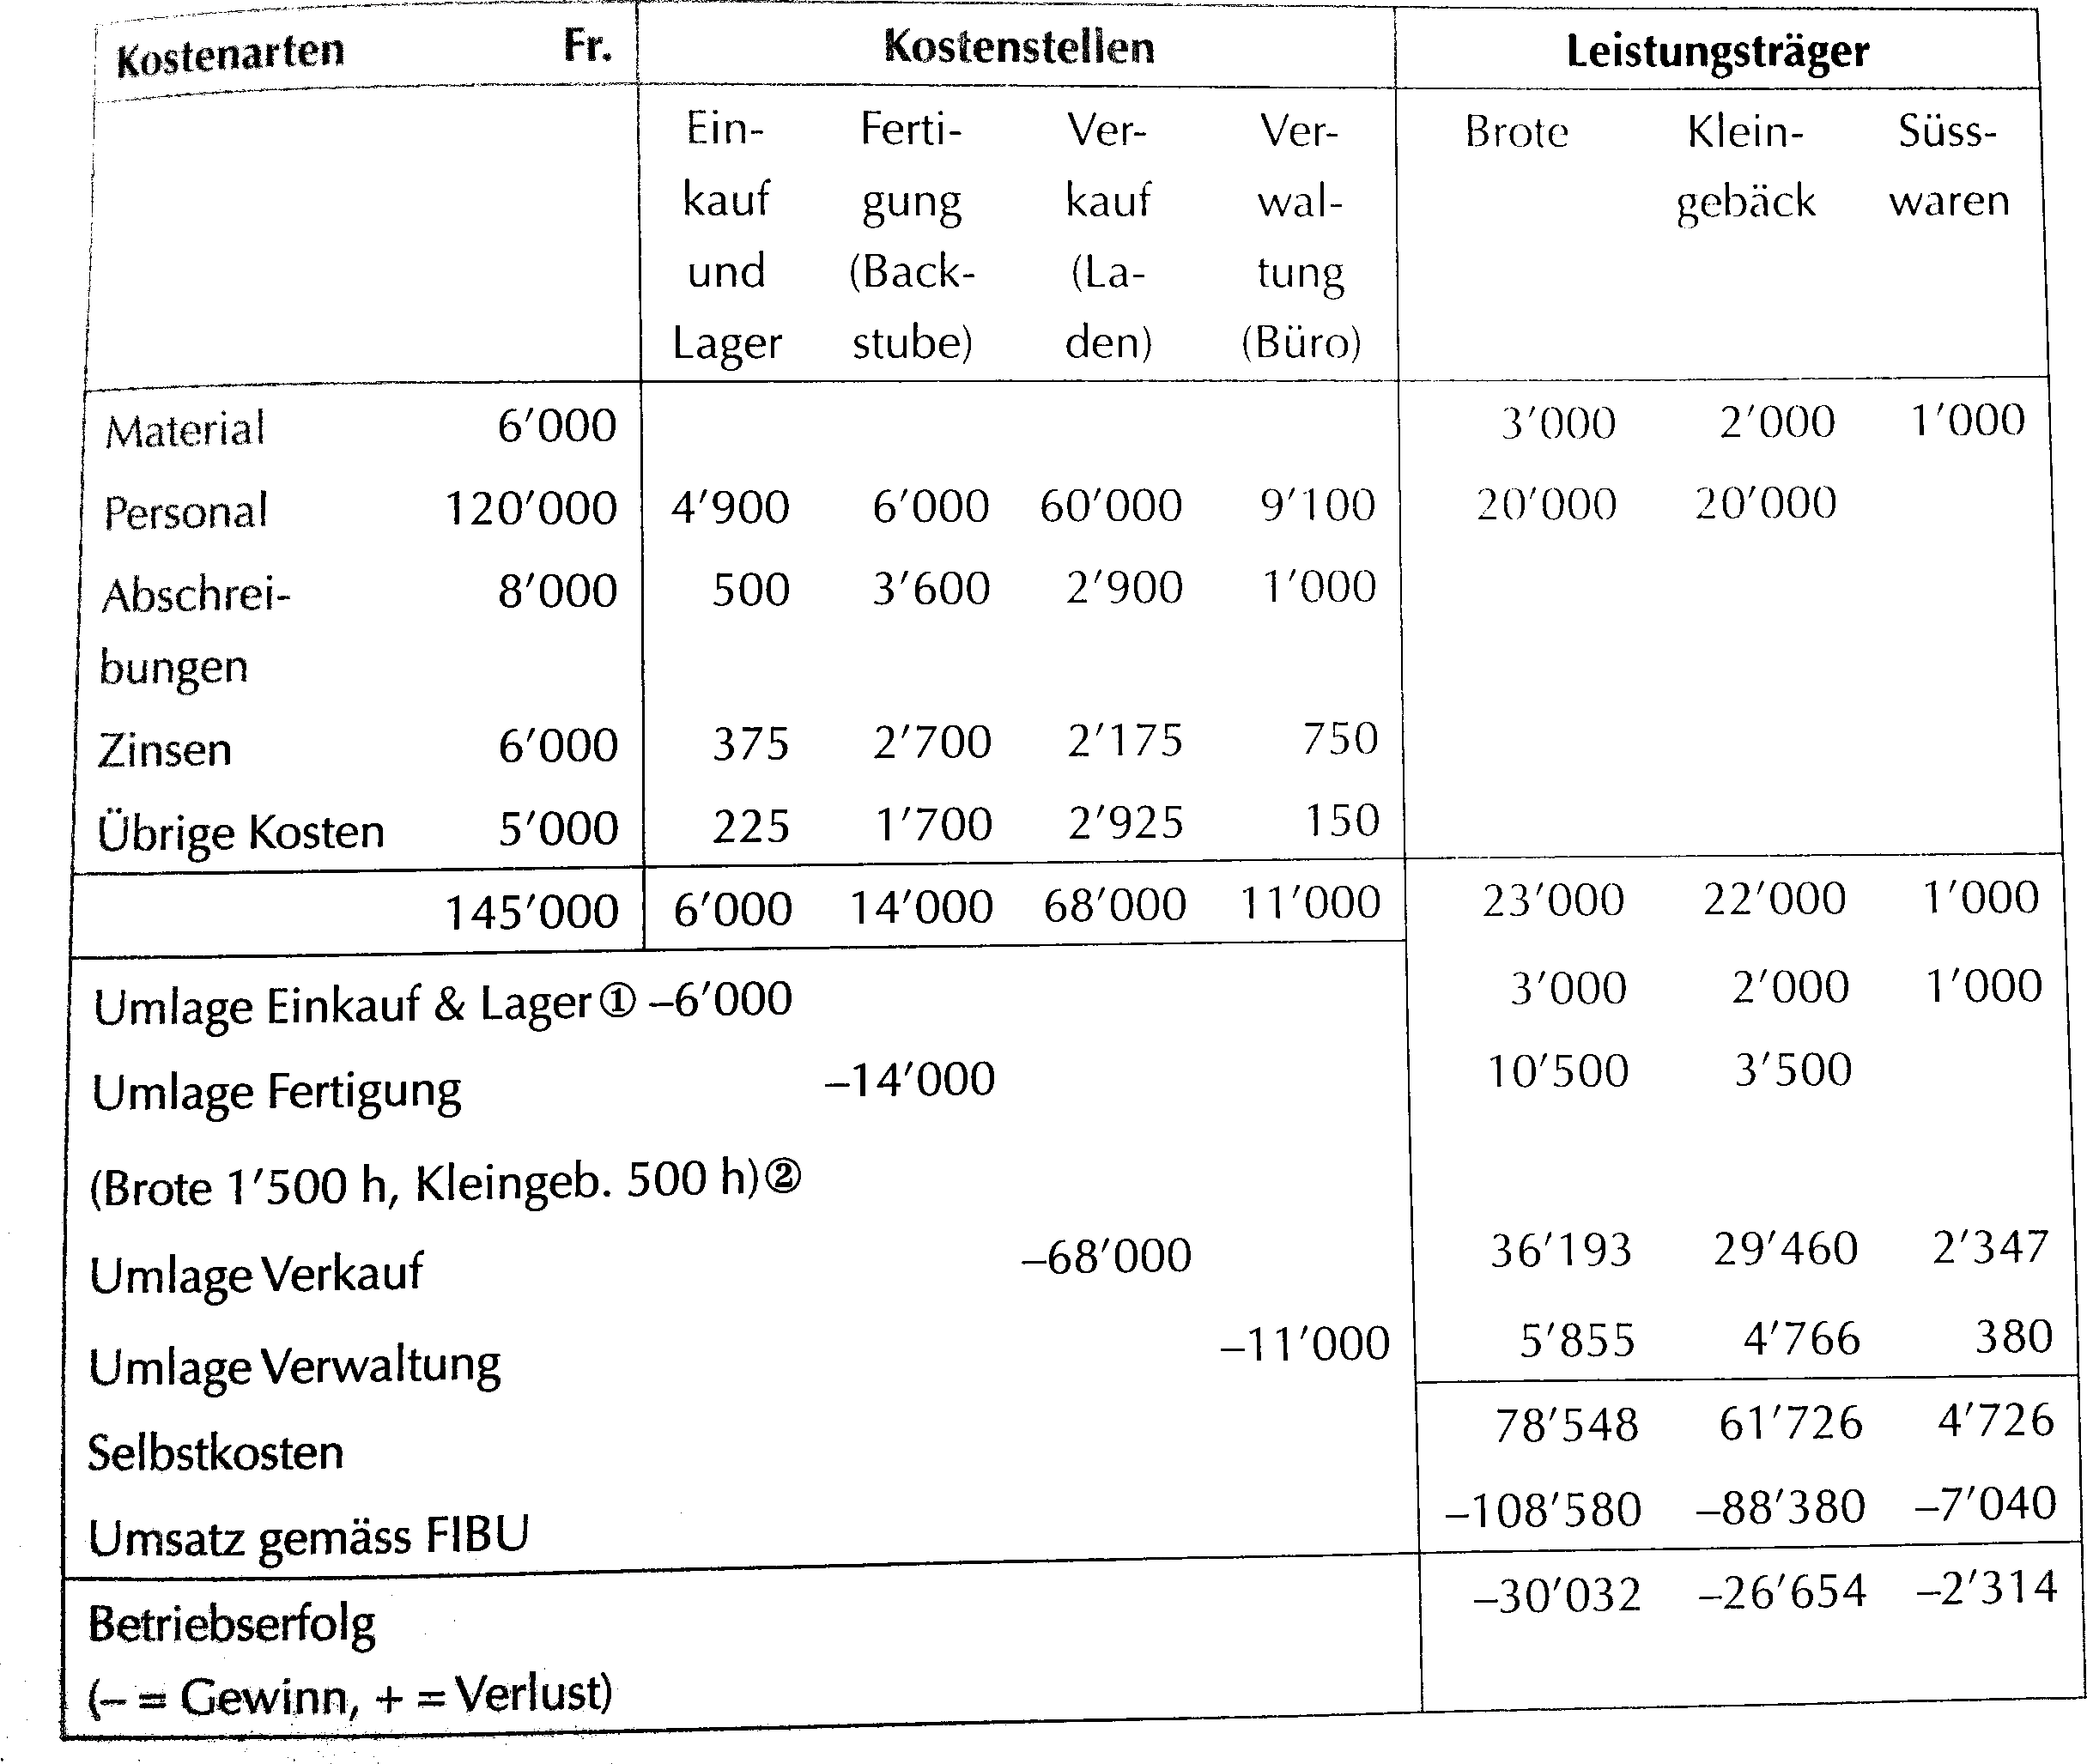
\includegraphics[scale=0.2]{KostenLeistungsrechnung/Kostenleistung}


\subsection*{Zurechnung der Kostenstellen}
\begin{itemize}
\item Einkauf und Lager $\frac{Einkauf\, und\, Lager}{Materialkoste}=\frac{6'000}{6'000}=100\%$
(1)
\item Fertigung $\frac{Fertigung}{Backstunden}=\frac{12'000}{2'000h}=7.00/h$
(1)
\item Verkauf $\frac{Verkauf}{Umsatz}=\frac{68'000}{204'000}=33.33\%$ (2)
\item Verwaltung $\frac{Verwaltung}{Umsatz}=\frac{11'000}{204'000}=5.39\%$
(2)\end{itemize}

